\label{chap4}

This chapter details the controller design of the model-based controller. The performance of the controller is tested with the aid of a simulation model. The model as derived in Chapter \ref{chap2} will be used with the parameters found in Chapter \ref{chap3}. First, the control layout is detailed. This schematically shows the control loop. Then, the model-based controller is detailed which comprises Jacobian information. Lastly, the pressure controller is detailed. 



\section{Control layout}

Figure \ref{fig4:controllayout} shows the schematic overview of the soft robot's control layout. This control architecture is detailed starting with the reference position vector $r_{set}$ containing the desired $x$ and $y$ coordinate. Based on the actual position $r_{est}$ in the Cartesian plane, position error $e_r$ can be determined. This error is injected into the model-based controller. This control law incorporates the current position through inverse kinematics. Based on the current configuration and position error, a control input $\nu_{set}$ is calculated. This control input can be viewed as a moment and force necessary to curve and elongate the soft robot. With the aid of some mapping, the input force and moment can be converted to a reference pressure's $p_{set}$ for each bellow. The difference between measured pressure $p$ and the reference pressure is defined as the pressure error $e_p$. Based on this pressure error, the pressure controller determines the volt input $V$ to the air pumps. The change in pressure affects position and orientation as perceived by the vision system and Inertial Measurement Unit (IMU), respectively. The measured Cartesian coordinates and rotation allows calculating the modal coordinates through inverse kinematics. These determined modal coordinates are then used to update the model-based controller. The measured Cartesian position will also be used to determine the position error. In this section, the control layout is further detailed. Starting with the model-based controller, then the pressure regulation.


\begin{figure}[H]
    \centering
    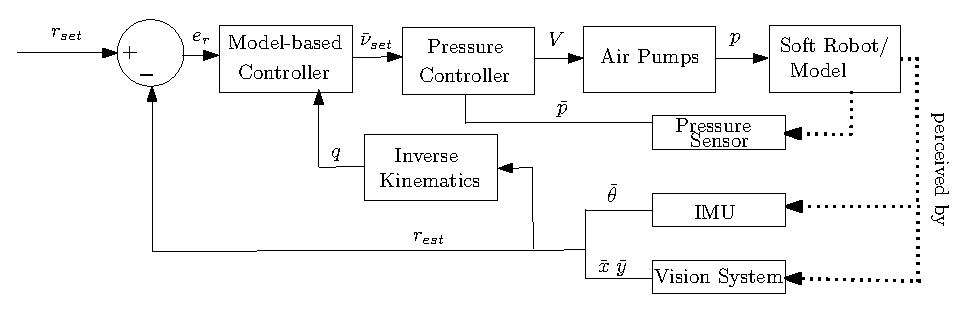
\includegraphics[width = \textwidth]{Figures/Chapter4/ControlschemeActualwithPump.eps}
    \caption{Control layout of the model-based controller accompanied by a low-level pressure controller.}
    \label{fig4:controllayout}
\end{figure}




\section{Jacobian model-based controller}


For controlling the soft robot, a model based controller is proposed based on the system's Jacobian matrix. As mentioned in Chapter \ref{chapter1}, Jacobian control has readily been applied to the field of soft robotics. In this work, a Jacobian controller is implemented based on \cite{MOOSAVIAN20071226}. The latter work states that a computed torque controller can be approximated by a more straightforward control law involving the Jacobian transpose. This approximation holds if high enough control gains are used. The work of \cite{MOOSAVIAN20071226} demonstrates this with a Jacobian PD controller. The control law that will be implemented is slightly altered. Since a PD controller has no integrator action, the steady-state error is not reduced. Furthermore, the presence of noise in the control loop does not lend itself for numeric differentiation, hence a standard derivative action can not be implemented. Therefore, a Jacobian PI controller will be implemented. The control law can then be formulated as,


\begin{equation}
    \nu_{set} = \begin{bmatrix}J_c(\sigma,t)\end{bmatrix}_1^\top \Big(K_p e_r + K_i \int_0^t e_r \hspace{2pt} ds \Big) \hspace{10pt} \text{with} \hspace{10pt} e_r = e_{set}-e_{est}, 
    \label{eq:tau}
\end{equation}

where $\nu_{set}$ is the desired control input, as calculated by the controller. Furthermore, the proportional-integrator structure can be directly observed. The diagonal gain matrices $K_p$ and $K_i$ both in $\mathbb{R}^{2\times 2}$ contain proportional and integrator gains, respectively. The proportional gain matrix $K_p$ penalizes proportional to the error, whereas integrator gain matrix $K_i$ contributes to the sum of the error over time. The error $e_r \in \mathbb{R}^2$ is defined as the difference between reference position $e_{set}$ and the measured position in the (x,y)-plane $e_{est}$. The Jacobian is determined with equation (\ref{eq2:J}) following a first-order approximation, as shown in Chapter \ref{chap3}. Since only the position in (x,y)-plane is considered, not the entire Jacobian of dimension $3 \times 2$ is used. Only the entries mapping modal coordinate position to Cartesian position are used. This corresponds to the second and third row of the Jacobian, which will be defined as $[J_c]_1$. Due to its space dependency, the Jacobian is updated in real-time based on the actual kinematic configuration of the actuator. Based on the measured position and angle the modal coordinates can be calculated using inverse kinematics. The simplified inverse kinematics are detailed in Appendix \ref{app4}.

Since the controller has a PI structure, oscillations in the control signal are not reduced as there is no derivative action in the control law. A derivative action could have easily been included based on numerical differentiation. However, this method is often erroneous velocity estimated due to the presence of noise. The origin of the noise comes from position measurement which, via inverse kinematics, also effects the calculation of the Jacobian. To reduce oscillation on the input signal, a low-pass filter is added to the controller law. The discretized low-pass filter is given as,

\begin{equation}
\bar{\nu}_{set,k} = \zeta \nu_{set,k} + (1-\zeta)\bar{\nu}_{set,k-1}
\label{eq4:lowpass}
\end{equation}

where $\zeta$ with $ 0 < \zeta \leq 1$ is a tuning parameter defining the relative importance between new input $\nu_{set,k}$ and previous input $\bar{\nu}_{set,k-1}$. A high value of $\zeta$ increases the cut-off frequency, resulting in minimal noise reduction. A low value for $\zeta$ suppresses more frequencies. Lowering the value of $\zeta$ increases the delays in the system, which can potentially cause stability problems. 


\section{Pressure control}


The actual system does not allow to induce forces and moments directly. Therefore the set control input $\nu_{set}$ should be mapped to some reference pressure. Using the inverse of the mapping found by finite element analysis in Chapter \ref{chap3} desired input forces and moments can be mapped to pressure. Based on the desired control input, a reference pressure can be formulated as,

\begin{equation}
    p_{set} = H^{-1}\bar{\nu}_{set},
\end{equation}


where $p_{set} \in \mathbb{R}^2$ is the reference pressure for each bellow. In order for this reference pressure to be reached a second controller is necessary. This low-level controller is used to set the input voltage that is supplied to the air pumps. A standard PI-controller is deemed good enough to track the reference pressure. Therefore the control law is can be described by,

\begin{equation}
    V = K_{pp}e_p + K_{ip} \int_0^t e_p \hspace{2pt} ds \hspace{10pt} \text{with} \hspace{10pt} e_p = p_{set} - p,
\end{equation}

where $V$ is the input voltage based on the pressure error $e_p$. The proportional action is based on diagonal gain matrix $K_{pp} \in \mathbb{R}^{2\times 2}$, whereas the integral action is done by $K_{ip} \in \mathbb{R}^{2\times 2}$.

















%\section{Digital Filters}


%Above state space model and presented Jacobian controller is implemented in \MATLAB. The used settings gains are $K_p = \text{diag}([400,400])$  and $K_i = \text{diag}([150,150])$. Figure  shows a simulation for a set point $q_{set} = [0 0.3]^\top$, which is equivalent to a position of [0,0.084]$m$ in the xy-plane.




%It is clear that since only a elongation is desired the pressure in both bellows should become equal. Therefore control input $V_1 = V_2$, and is saturated to the maximum 12V. Once the setpoint is nearly reached the control input slowly drops to ... V. It can be seen that the pump dynamics are the major limiting factor in the achievable performance of the set-up. The dynamic model simulations shown in Appendix \ref{app4} showed that for a free oscillation the settling time is in the order of 0.1 seconds. For this setpoint the settling time is around ... seconds. Clearly the actuator damping does not play a large role setpoint regulation. . As one can see the controller  


%Using the same tuning parameters a curvature set-point as $q_{set} = [10,0.3]$ can be simulated. 


%\begin{figure}
%    \centering
%    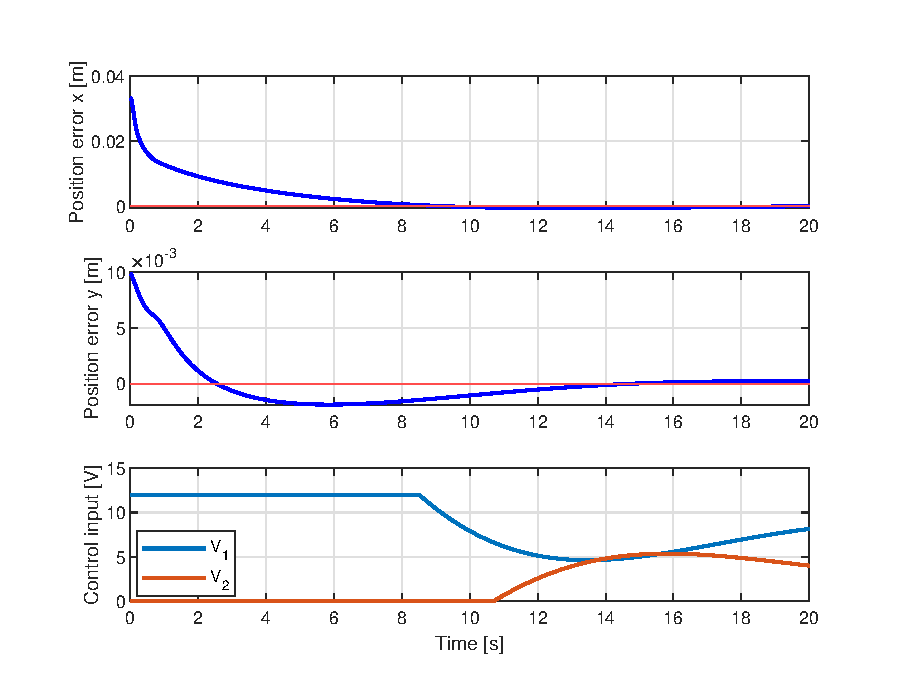
\includegraphics{Figures/Chapter4/k10e03.eps}
 %   \caption{Caption}
%    \label{fig:my_label}
%\end{figure}


























%The proposed Jacobian controller can be improved by adding additional model information. A major improving factor to the performance of the controller is adding stiffness compensation. Since the set-point is known, the necessary stiffness force and moment at that position are known. This compensation can directly be added to the control signal. The resulting controller then is,


%\begin{equation}
  %  \tau_{set} = \begin{bmatrix}J(\sigma,t)\end{bmatrix}^\top \Big(K_p e %+ K_i \int_0^t e \hspace{2pt} ds +  K_d \dot{e}\Big) + %\begin{bmatrix} K_\kappa(\kappa_{set}) & 0 \\ 0 & %K_\epsilon(\epsilon_{set}) \end{bmatrix} q_{set} , 
%    \label{eq:tauK}
%\end{equation}

%where additionally the stiffness is evaluated at modal coordinate setpoint $q_{set}$